\apendice{Documentación de usuario}

\section{Introducción}

En este apartado se presenta el manual de usuario de la aplicación, describiendo los requisitos mínimos necesarios para acceder al sistema y utilizar sus principales funcionalidades, así como un índice de instalación de las herramientas necesarias y los pasos a seguir para entender las funcionalidades más simples. El objetivo es que cualquier usuario pueda comprender las condiciones básicas de uso antes de interactuar con la herramienta.

\section{Requisitos de usuarios}

Para utilizar correctamente la aplicación no se requiere instalar ningún programa específico en el equipo del usuario, ya que el acceso se realiza mediante navegador web. No obstante, sí es necesario cumplir una serie de requisitos básicos que garanticen el correcto funcionamiento de la interfaz, del visor cartográfico y de las opciones de descarga.

\begin{itemize}
	\item \textbf{Dispositivo con navegador web:} se necesita un ordenador, portátil o dispositivo equivalente capaz de acceder a una aplicación web.
	
	\item \textbf{Navegador actualizado:} se recomienda emplear Google Chrome, Mozilla Firefox, Microsoft Edge, Safari u otro navegador moderno compatible con HTML5, CSS y JavaScript.
	
	\item \textbf{JavaScript habilitado:} la aplicación utiliza JavaScript para gestionar la interacción con la interfaz, el visor cartográfico, la colección de imágenes, los modales y diversos controles visuales.
	
	\item \textbf{Conexión a internet:} es necesaria para acceder al servidor donde se encuentre alojada la aplicación y, en su caso, para cargar los recursos cartográficos utilizados por el visor.
	
	\item \textbf{Pantalla y dispositivo de entrada:} se requiere una pantalla y un medio de interacción, como teclado y ratón o panel táctil, para utilizar formularios, botones, menús, mapas y galerías.
	
	\item \textbf{Permiso de descarga en el navegador:} debe permitirse la descarga de archivos para obtener imágenes procesadas, ficheros \texttt{ZIP} o resultados generados por la aplicación.
\end{itemize}

\section{Instalación}
%Redactar

\section{Manual del usuario}

Este manual será utilizado por aquellos usuarios que accedan de forma anónima a la aplicación o se registren en la misma, ya que los administradores contarán con sus indicaciones propias.

\subsection{Página principal y cálculo de trazas}

La página principal constituye el flujo más básico de la aplicación. Desde esta pantalla el usuario puede seleccionar una imagen aérea, ejecutar el cálculo de trazas de herbivoría y visualizar el resultado directamente sobre la imagen original.

\begin{figure}[]
	\centering
	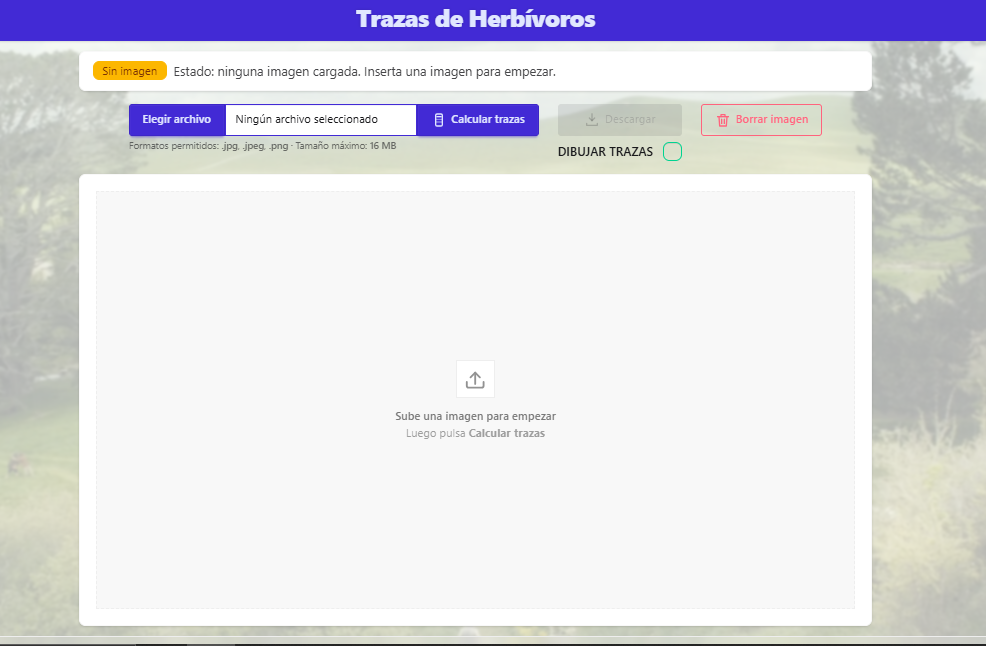
\includegraphics[width=\textwidth]{img/Home_sin_imagen}
	\caption[Página principal sin imagen cargada]{Página principal de la aplicación antes de seleccionar una imagen.}
	\label{fig:manual_home_sin_imagen}
\end{figure}

Al acceder a la página, la aplicación muestra un área central vacía destinada a la previsualización de la imagen, como se observa en la Figura~\ref{fig:manual_home_sin_imagen}. Para cargar una imagen, el usuario puede pulsar el botón \textit{Elegir archivo} o hacer clic sobre el cuadro grande situado en la zona central de la pantalla. Los formatos admitidos son \texttt{.jpg}, \texttt{.jpeg} y \texttt{.png}. En este primer paso la imagen solo se muestra en la interfaz para que el usuario pueda comprobar que ha seleccionado el fichero correcto. Cabe aclarar que, dicha imagen, no se guarda todavía en el sistema por si hubiese habido algún fallo a la hora de ser seleccionada.

\begin{figure}[]
	\centering
	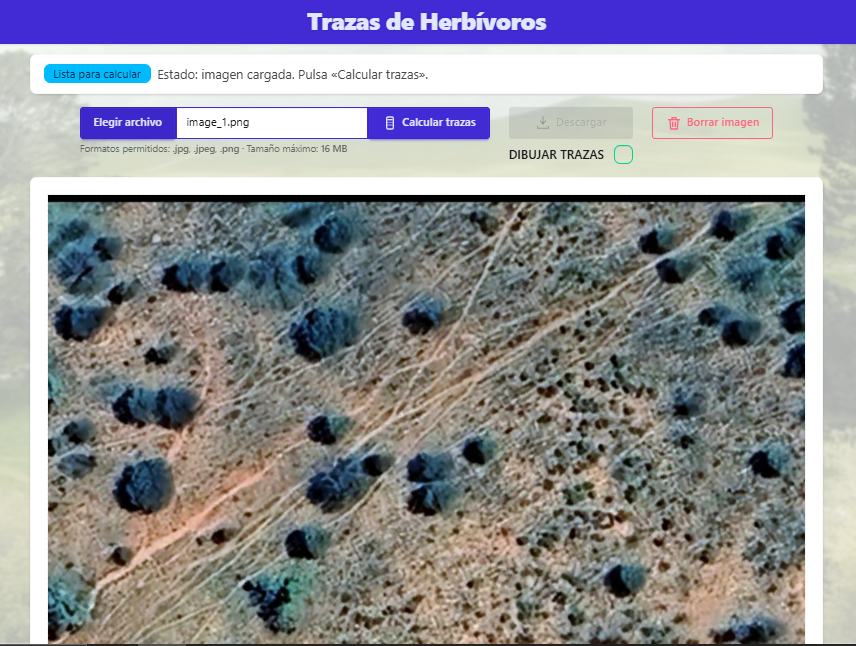
\includegraphics[width=\textwidth]{img/Home_con_imagen}
	\caption[Página principal con imagen cargada]{Página principal tras seleccionar una imagen aérea para su análisis.}
	\label{fig:manual_home_con_imagen}
\end{figure}

Una vez seleccionada la imagen, esta aparece en el área de previsualización, tal y como se muestra en la Figura~\ref{fig:manual_home_con_imagen}, y se habilita el flujo de cálculo. Para iniciar el procesamiento, el usuario debe pulsar el botón \textit{Calcular trazas}. En ese momento, la aplicación guarda la imagen y comienza el análisis. Mientras se realiza el cálculo, se muestra un modal informativo con el mensaje de cálculo de trazas y un icono de carga, indicando que el sistema está trabajando y que el usuario debe esperar a que finalice el proceso.

\begin{figure}[]
	\centering
	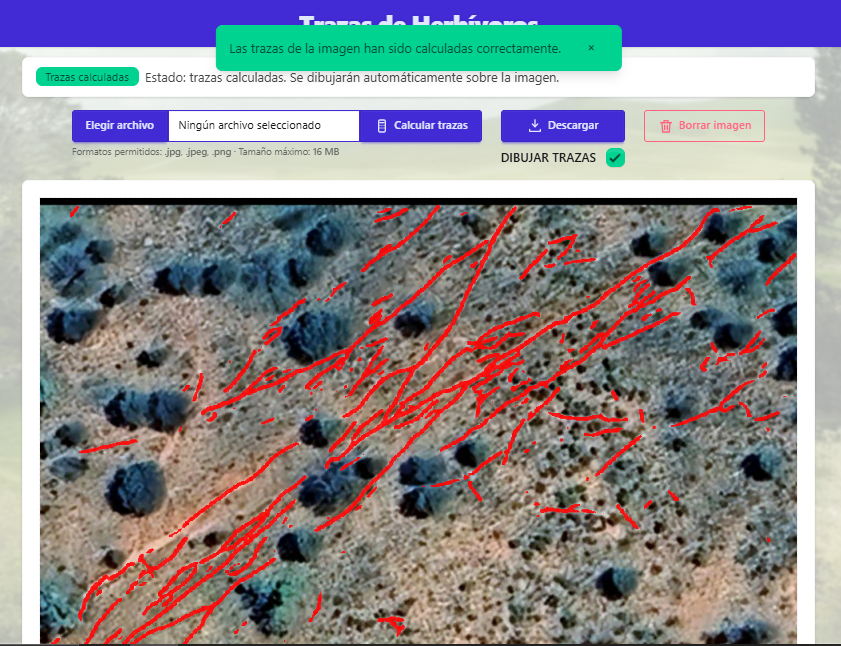
\includegraphics[width=\textwidth]{img/Home_con_trazas}
	\caption[Página principal con trazas calculadas]{Visualización de la imagen con las trazas calculadas y superpuestas en rojo.}
	\label{fig:manual_home_con_trazas}
\end{figure}

Cuando el cálculo termina correctamente, la aplicación muestra un aviso de confirmación y representa las trazas detectadas en color rojo sobre la imagen, como se aprecia en la Figura~\ref{fig:manual_home_con_trazas}. El \textit{checkbox} de \textit{Dibujar trazas} permite alternar la visualización del resultado: si está marcado, las trazas aparecen superpuestas sobre la imagen; si se desmarca, se muestra únicamente la imagen original sin la capa de trazas.

El botón \textit{Descargar} permanece deshabilitado hasta que la imagen ha sido procesada y las trazas se encuentran disponibles. Una vez habilitado, permite descargar un fichero \texttt{ZIP} que contiene la imagen original, el resultado generado y el archivo \texttt{JSON} con la información de las trazas. Por otro lado, el botón \textit{Borrar imagen} permite limpiar la imagen cargada y devolver la pantalla a su estado inicial.

Si el usuario intenta calcular trazas o borrar una imagen sin haber cargado previamente ningún fichero, la aplicación mostrará un mensaje de error. De este modo se evita ejecutar operaciones inválidas y se mantiene un flujo de uso claro: primero seleccionar la imagen, después calcular las trazas y, finalmente, visualizar o descargar los resultados.

\subsection{Registro, inicio y cierre de sesión}

La aplicación permite trabajar tanto como usuario anónimo, como con una cuenta registrada. El uso como visitante permite acceder al flujo básico de carga de imágenes y cálculo de trazas, mientras que el registro habilita funcionalidades asociadas a una cuenta, como la gestión del perfil, el acceso al visor cartográfico, la consulta de colecciones persistentes y, en función del rol, las opciones de administración.

\begin{figure}[]
	\centering
	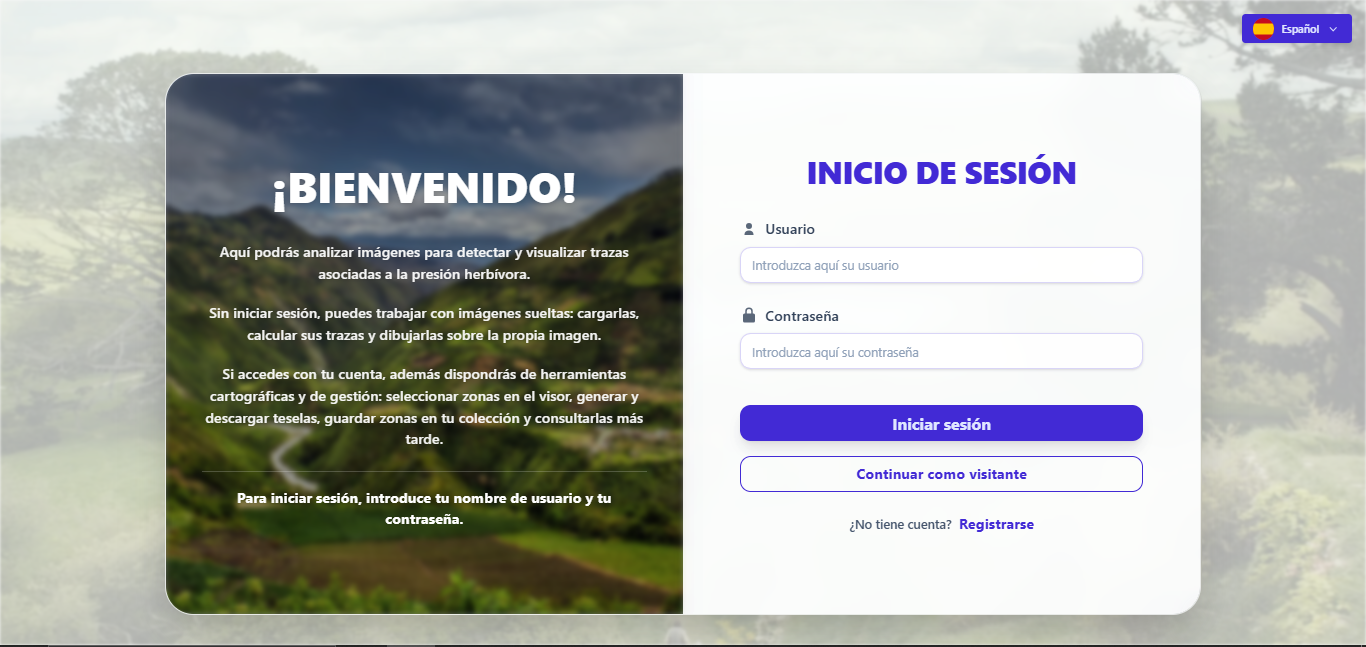
\includegraphics[width=\textwidth]{img/Página_log_in}
	\caption[Página de inicio de sesión]{Página de inicio de sesión de la aplicación.}
	\label{fig:manual_login}
\end{figure}

La pantalla de inicio de sesión, mostrada en la Figura~\ref{fig:manual_login}, permite acceder a la aplicación mediante un nombre de usuario y una contraseña. En esta misma vista se ofrece también la posibilidad de continuar como visitante, opción pensada para usuarios que desean probar el funcionamiento básico de la herramienta sin crear una cuenta. Además, desde esta pantalla se puede acceder al formulario de registro mediante el enlace \textit{Registrarse}.

\begin{figure}[]
	\centering
	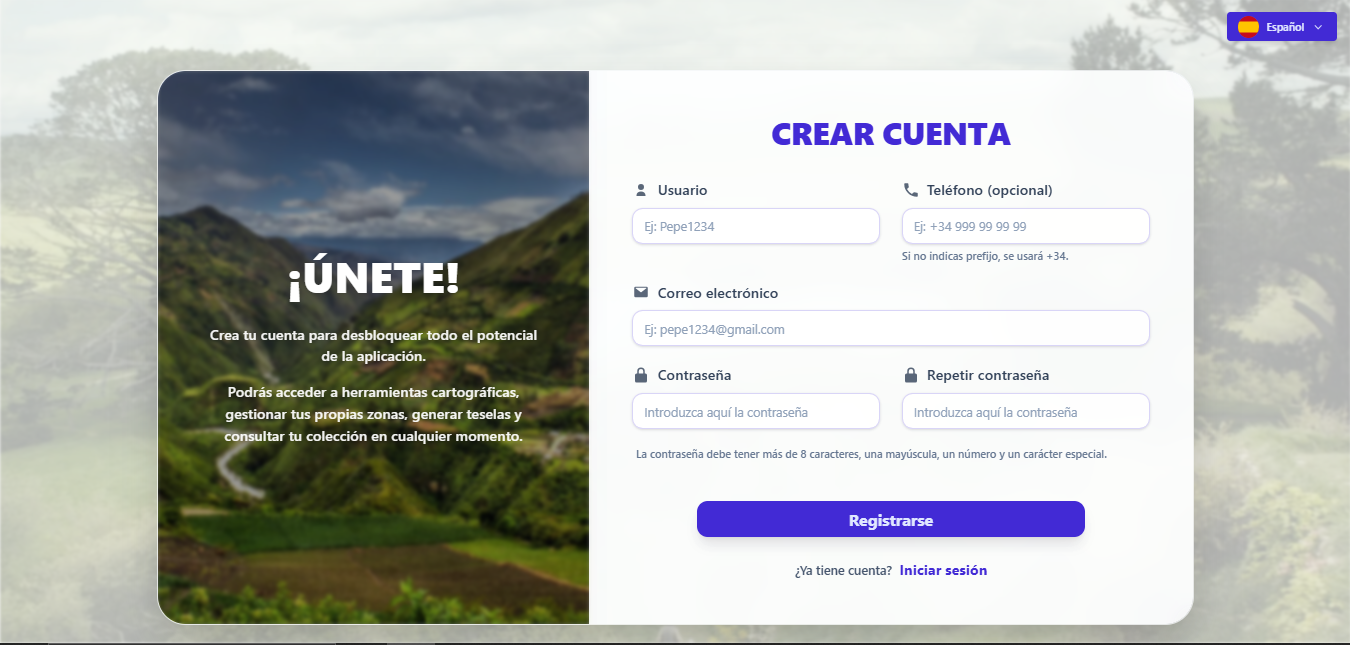
\includegraphics[width=\textwidth]{img/Página_registro}
	\caption[Página de registro]{Formulario de creación de una nueva cuenta de usuario.}
	\label{fig:manual_registro}
\end{figure}

Para crear una cuenta nueva, el usuario debe completar el formulario de registro representado en la Figura~\ref{fig:manual_registro}. En esta página se solicita un nombre de usuario, un correo electrónico, una contraseña, la repetición de dicha contraseña y, de forma opcional, un número de teléfono. El correo electrónico debe presentar un formato válido, incluyendo el símbolo \texttt{@} y un dominio correcto, como \texttt{@gmail.com}, \texttt{@hotmail.com} u otro equivalente. La contraseña debe cumplir unos requisitos mínimos de seguridad: tener más de ocho caracteres e incluir al menos una letra mayúscula, un número y un carácter especial. Además, los campos de contraseña y repetición de contraseña deben coincidir para poder completar el registro.

Una vez creada la cuenta, el usuario puede iniciar sesión desde la pantalla anterior introduciendo sus credenciales. Si los datos son correctos, la aplicación carga la interfaz principal asociada al usuario autenticado. A partir de ese momento, el menú lateral cambia para mostrar las opciones disponibles según el tipo de usuario.

\begin{figure}[]
	\centering
	\includegraphics[width=\textwidth]{img/usuario_visitante}
	\caption[Menú de usuario visitante]{Menú lateral mostrado cuando se accede como usuario visitante.}
	\label{fig:manual_usuario_visitante}
\end{figure}

Cuando se trabaja como un usuario anónimo, tal y como se observa en la Figura~\ref{fig:manual_usuario_visitante}, el menú lateral muestra las opciones básicas de navegación y mantiene disponible el acceso a inicio de sesión. Este modo permite utilizar la funcionalidad principal de la aplicación sin asociar los resultados a una cuenta persistente, por lo que no se dispone de perfil propio ni de gestión de colecciones personales.

\begin{figure}[]
	\centering
	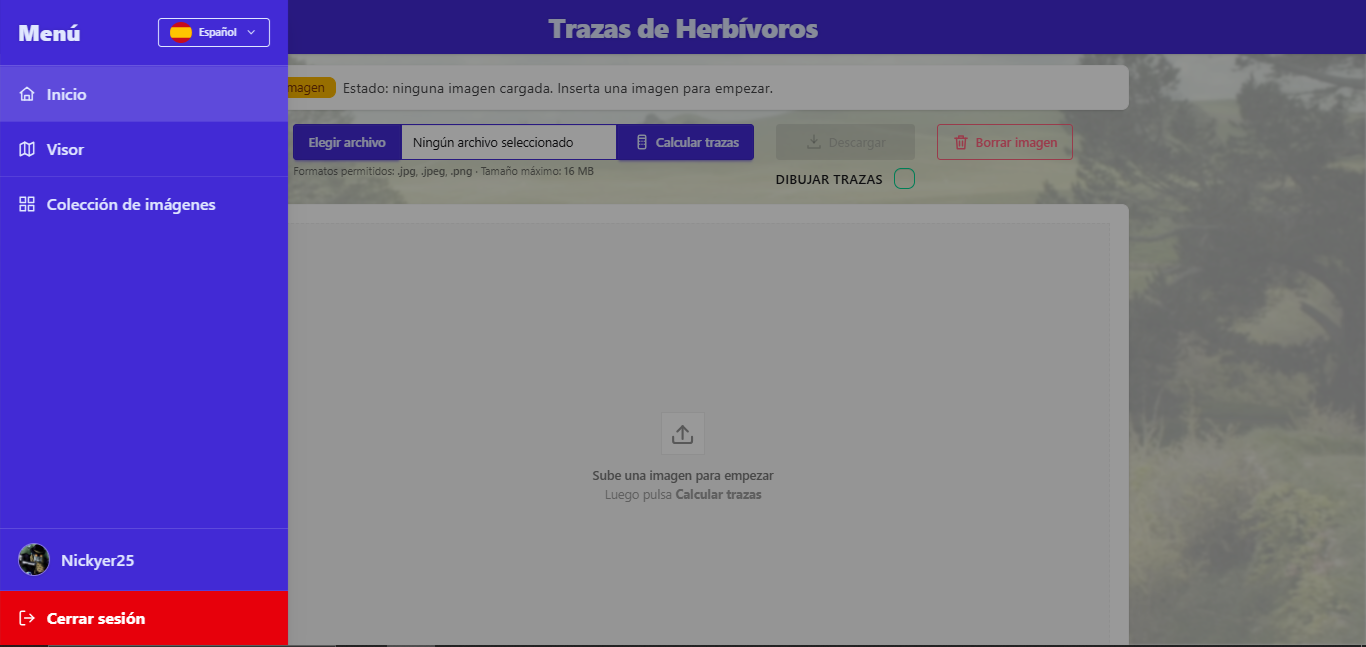
\includegraphics[width=\textwidth]{img/Página_usuario}
	\caption[Menú de usuario registrado]{Menú lateral mostrado para un usuario registrado.}
	\label{fig:manual_usuario_registrado}
\end{figure}

En el caso de un usuario registrado, el menú lateral incorpora el nombre y la imagen de perfil del usuario, además de las opciones de navegación propias de una cuenta autenticada. Como se aprecia en la Figura~\ref{fig:manual_usuario_registrado}, desde este menú se puede acceder a la página principal, al visor cartográfico, a la colección de imágenes y al perfil. También se incluye la opción \textit{Cerrar sesión}, que finaliza la sesión activa y devuelve al usuario al estado no autenticado.

\begin{figure}[]
	\centering
	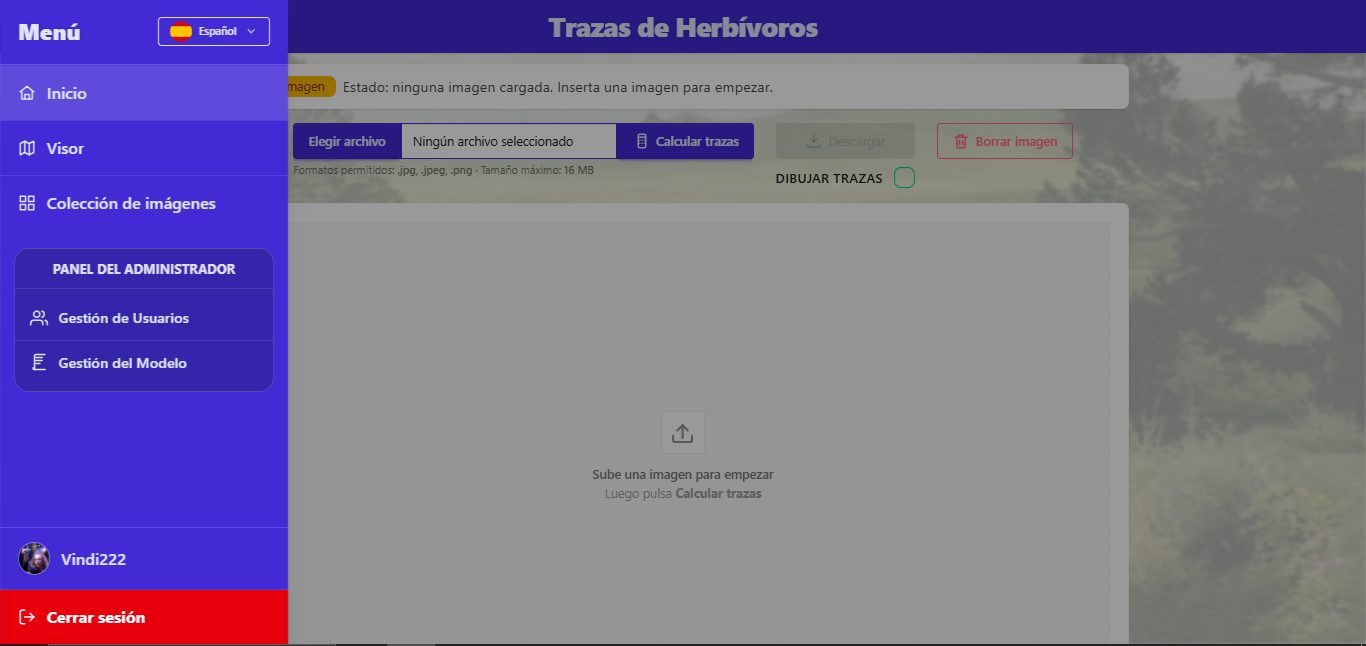
\includegraphics[width=\textwidth]{img/Página_administrador}
	\caption[Menú de administrador]{Menú lateral mostrado para un usuario con permisos de administración.}
	\label{fig:manual_administrador}
\end{figure}

La principal diferencia entre un usuario normal y un administrador se encuentra en la disponibilidad del panel de administración. En la Figura~\ref{fig:manual_administrador} se observa que, además de las opciones generales de navegación, el administrador dispone de accesos específicos para la gestión de usuarios y la gestión del modelo. Estas opciones permiten realizar tareas de mantenimiento del sistema, por lo que solo están visibles y disponibles para cuentas con rol de administrador.

Para cerrar sesión, el usuario debe abrir el menú lateral y pulsar la opción \textit{Cerrar sesión}. Al hacerlo, la aplicación finaliza la sesión actual y vuelve a mostrar las opciones correspondientes a un usuario no autenticado.

\subsection{Perfil de usuario e imagen de perfil}

El perfil de usuario permite consultar la información asociada a la cuenta y modificar algunos de sus datos personales. A esta pantalla se accede desde el menú lateral, mediante la opción \textit{Perfil}, disponible para usuarios registrados. En ella se muestran el nombre de usuario, el correo electrónico, el teléfono, la fecha de alta y la imagen de perfil, además de accesos rápidos al visor, a la colección de imágenes y, en el caso de los administradores, a las secciones de gestión correspondientes.

\begin{figure}[]
	\centering
	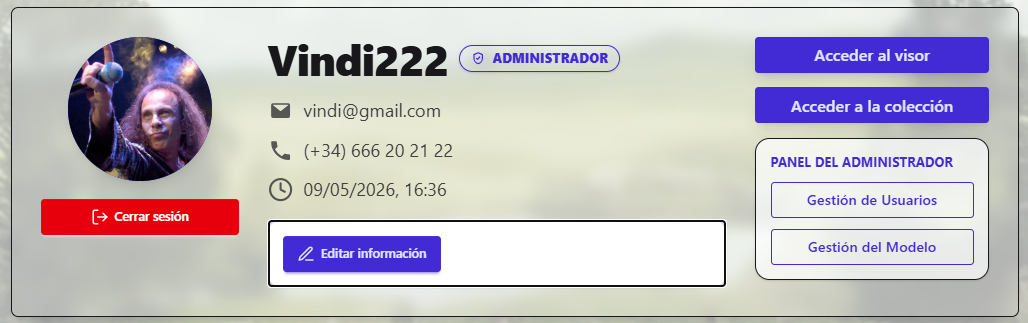
\includegraphics[width=\textwidth]{img/Página_perfil}
	\caption[Página de perfil de usuario]{Página de perfil con la información principal de la cuenta.}
	\label{fig:manual_perfil}
\end{figure}

Como se observa en la Figura~\ref{fig:manual_perfil}, la pantalla de perfil centraliza la información principal del usuario y permite realizar acciones relacionadas con la cuenta. Si el usuario no ha configurado una imagen personalizada, la aplicación muestra un avatar genérico. En caso contrario, se utiliza la imagen de perfil seleccionada, que también aparece en el menú lateral junto al nombre de usuario, facilitando la identificación de la sesión activa.

Para modificar los datos personales, el usuario debe pulsar el botón \textit{Editar información}. Al hacerlo, se despliega un formulario en el que pueden cambiarse campos como el nombre de usuario, el correo electrónico o el teléfono, tal y como se muestra en la Figura~\ref{fig:manual_editar_perfil}. Una vez introducidos los nuevos valores, el usuario debe pulsar \textit{Guardar cambios} para actualizar la información de la cuenta.

\begin{figure}[]
	\centering
	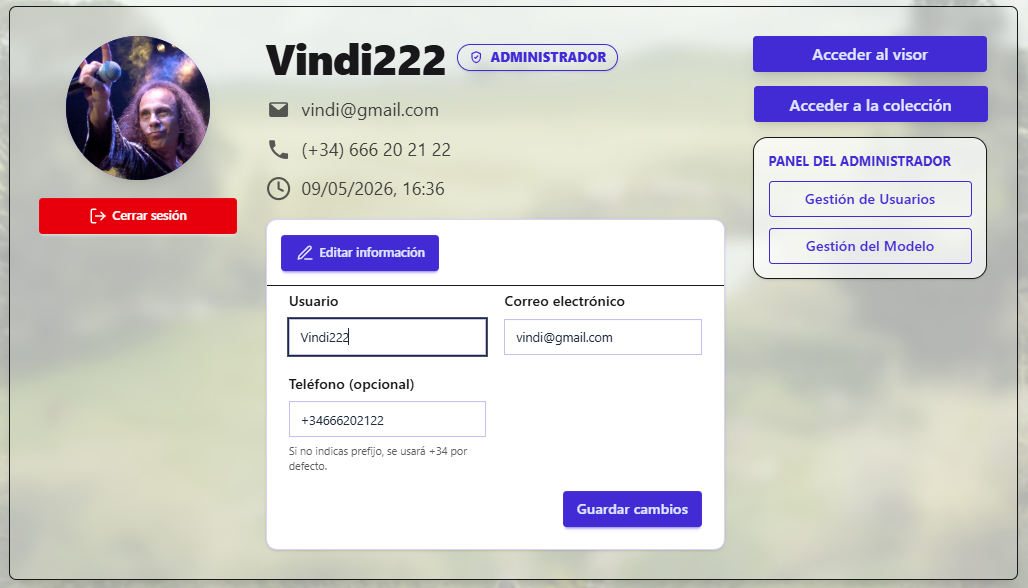
\includegraphics[width=\textwidth]{img/Editar_información}
	\caption[Edición de información del perfil]{Formulario de edición de los datos personales del usuario.}
	\label{fig:manual_editar_perfil}
\end{figure}

La aplicación también permite cambiar la imagen asociada al perfil. Para ello, el usuario selecciona una nueva imagen desde la pantalla de perfil. Antes de guardarla definitivamente, el sistema muestra una pantalla de confirmación, representada en la Figura~\ref{fig:manual_confirmar_imagen_perfil}. Esta vista permite comprobar que la imagen se visualiza correctamente y que el recorte circular del avatar es adecuado antes de aplicar el cambio.

\begin{figure}[]
	\centering
	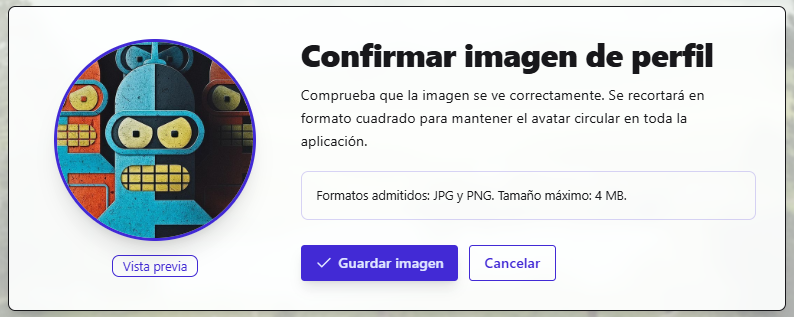
\includegraphics[width=\textwidth]{img/Cambio_img_perfil}
	\caption[Confirmación de imagen de perfil]{Pantalla de confirmación previa al guardado de una nueva imagen de perfil.}
	\label{fig:manual_confirmar_imagen_perfil}
\end{figure}

Esta confirmación evita que se guarden imágenes incorrectas o mal encuadradas sin revisión previa. Si el usuario acepta el cambio, la nueva imagen queda asociada a la cuenta y se actualiza tanto en la página de perfil como en el menú lateral. Si cancela la operación, se mantiene la imagen anterior y no se modifica la información de la cuenta.

\subsection{Visor cartográfico}

El visor cartográfico permite seleccionar una zona sobre el mapa para generar una cuadrícula de teselas que posteriormente podrá procesarse como una colección de imágenes. Esta funcionalidad está pensada para trabajar con áreas geográficas completas, de forma que el usuario pueda delimitar una región de interés y dejar que la aplicación genere automáticamente las imágenes necesarias para su análisis.

\begin{figure}[]
	\centering
	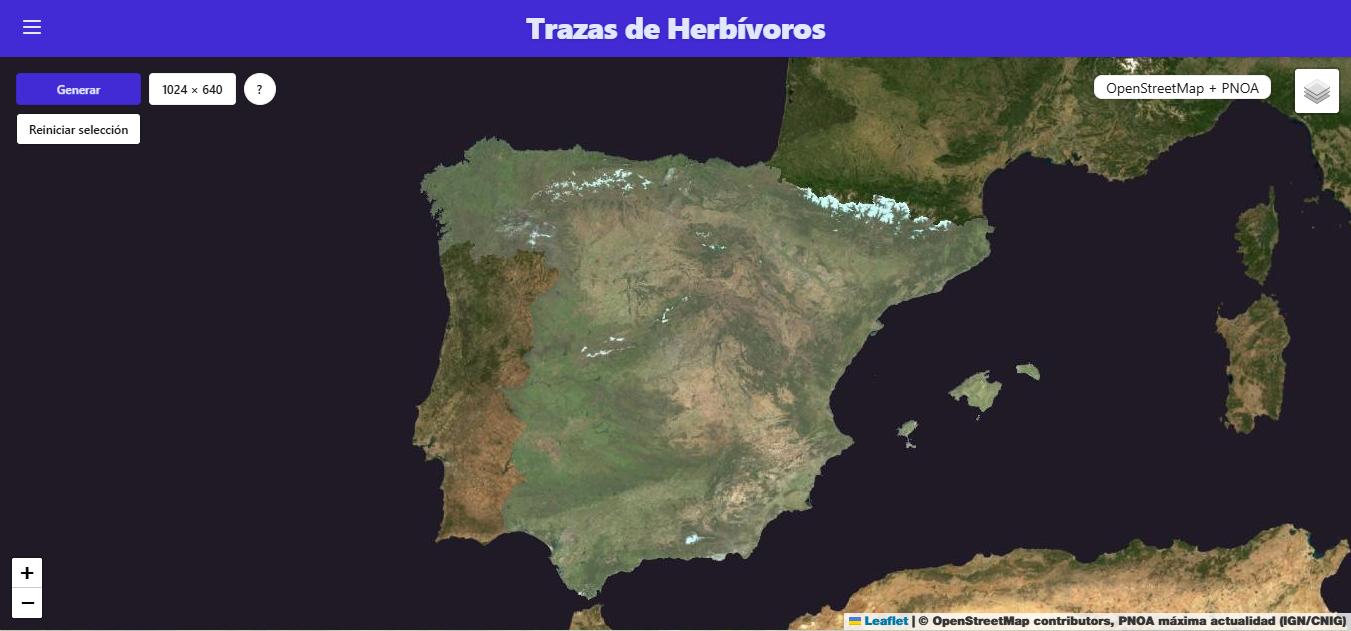
\includegraphics[width=\textwidth]{img/Página_visor}
	\caption[Visor cartográfico]{Vista inicial del visor cartográfico con controles de generación, resolución y ayuda.}
	\label{fig:manual_visor}
\end{figure}

Para acceder al visor, el usuario debe seleccionar la opción \textit{Visor} desde el menú lateral. Como se observa en la Figura~\ref{fig:manual_visor}, la pantalla muestra un mapa interactivo junto con los controles principales de trabajo. El usuario puede desplazarse por el mapa manteniendo pulsado el cursor y arrastrando la pantalla. También puede ampliar o reducir la escala mediante los botones de \textit{zoom} situados en el mapa o utilizando la rueda del ratón.

El flujo de uso comienza seleccionando dos puntos sobre el mapa. Estos puntos definen un área rectangular que será utilizada por la aplicación para calcular la cuadrícula de teselas. Si el usuario se equivoca al marcar la zona, puede pulsar el botón \textit{Reiniciar selección}, que elimina los puntos seleccionados y permite comenzar de nuevo sin generar ninguna colección.

En la parte superior del visor se encuentra el botón \textit{Generar}, el selector de resolución objetivo y un botón de ayuda identificado con un signo de interrogación. Este último, junto con las etiquetas informativas de la interfaz, orienta al usuario sobre los pasos necesarios para completar correctamente la selección y generación de la zona.

\begin{figure}[]
	\centering
	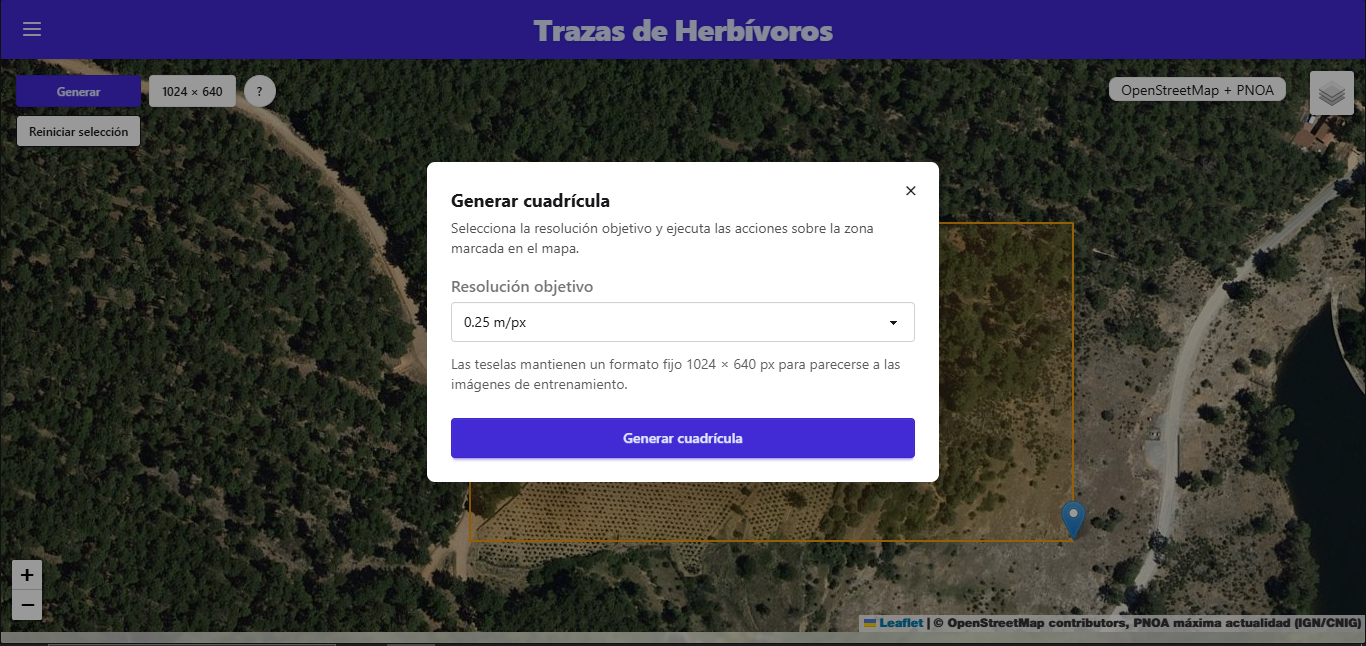
\includegraphics[width=\textwidth]{img/Generar_cuadrícula_visor}
	\caption[Modal de generación de cuadrícula]{Modal de generación de cuadrícula a partir de la zona seleccionada en el visor.}
	\label{fig:manual_generar_cuadricula}
\end{figure}

Una vez marcada una zona válida, el usuario debe pulsar el botón \textit{Generar}. En ese momento se abre el modal mostrado en la Figura~\ref{fig:manual_generar_cuadricula}, donde se puede seleccionar la resolución objetivo de las teselas. Esta resolución condiciona el nivel de detalle de las imágenes generadas y, por tanto, también el tiempo necesario para completar la operación. Tras confirmar mediante el botón \textit{Generar cuadrícula}, la aplicación calcula las teselas correspondientes a la zona seleccionada.

La zona seleccionada debe ser válida para que el proceso pueda completarse. En particular, no debe situarse fuera de los límites admitidos ni corresponder a áreas no adecuadas para el análisis, como zonas marítimas. Si la selección no cumple las condiciones necesarias, la aplicación informará del problema y solicitará al usuario que modifique el área antes de continuar.

\begin{figure}[]
	\centering
	\includegraphics[width=\textwidth]{img/cuadrícula_generada}
	\caption[Cuadrícula generada desde el visor]{Zona registrada correctamente y listado de teselas generadas para la colección.}
	\label{fig:manual_cuadricula_generada}
\end{figure}

Cuando la cuadrícula se genera correctamente, la aplicación muestra un mensaje de confirmación y ofrece la opción de abrir la colección creada, tal y como se aprecia en la Figura~\ref{fig:manual_cuadricula_generada}. En esta vista se muestra también la lista de teselas generadas, que pueden descargarse de forma individual o conjunta mediante un fichero \texttt{ZIP}. Desde el botón \textit{Abrir colección}, el usuario puede acceder directamente a la colección asociada a la zona seleccionada para consultar el estado de procesamiento y visualizar posteriormente los resultados.

El tiempo de generación puede variar en función del tamaño de la zona seleccionada, la resolución elegida y la disponibilidad de los servicios cartográficos utilizados. Por ello, se recomienda seleccionar áreas ajustadas al análisis que se desea realizar, evitando zonas excesivamente grandes si no son necesarias.

\subsection{Colección de imágenes}

La sección de colección de imágenes muestra las zonas generadas previamente desde el visor cartográfico y permite consultar el estado de procesamiento de sus teselas. Desde esta pantalla el usuario puede revisar sus colecciones, acceder a la galería de imágenes, volver a visualizar una zona sobre el mapa, descargar resultados y gestionar las colecciones creadas.

\begin{figure}[]
	\centering
	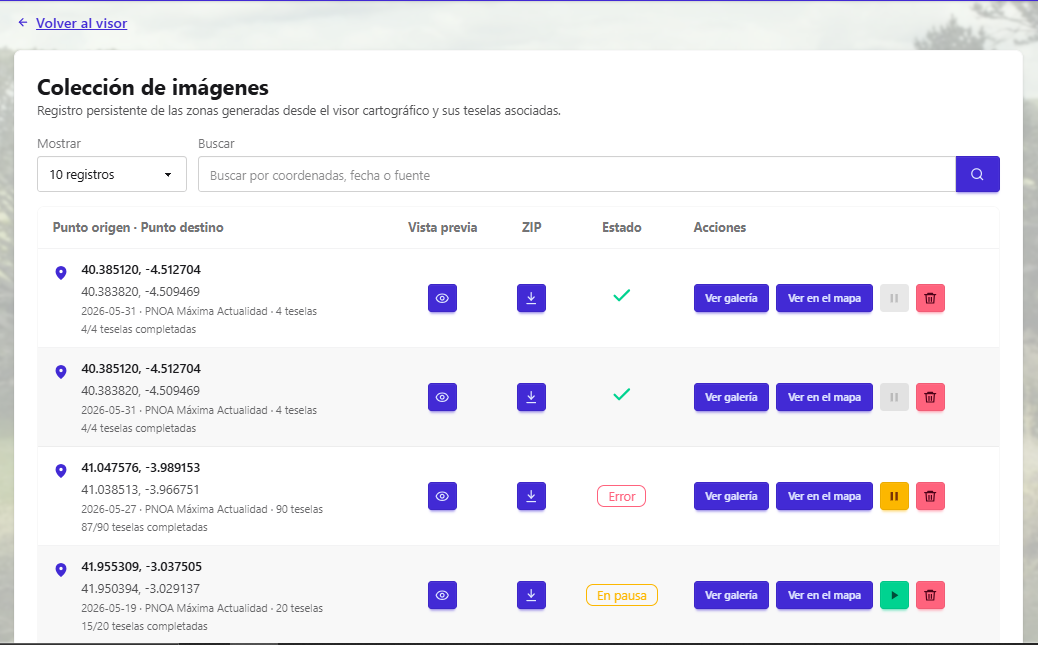
\includegraphics[width=\textwidth]{img/Página_colección}
	\caption[Colección de imágenes]{Listado de colecciones generadas desde el visor cartográfico.}
	\label{fig:manual_coleccion}
\end{figure}

Como se observa en la Figura~\ref{fig:manual_coleccion}, cada colección aparece representada en una tabla con información sobre la zona seleccionada, la fecha de creación, la fuente cartográfica utilizada, el número de teselas generadas y el progreso del procesamiento. En la parte superior se incluye un selector para modificar el número de registros visibles y un buscador que permite localizar colecciones a partir de sus coordenadas, fecha o fuente.

Cada fila de la tabla incorpora un indicador de estado. Una colección puede encontrarse en estado pendiente, cuando todavía no se ha iniciado el procesamiento; procesando, cuando sus teselas se están calculando; completada, cuando todas las imágenes han terminado correctamente; pausada, cuando el usuario ha detenido temporalmente el procesamiento; o error, cuando alguna operación no se ha podido completar. Además, se muestra el número de teselas completadas respecto al total, lo que permite conocer el avance sin necesidad de entrar en la galería.

\begin{figure}[]
	\centering
	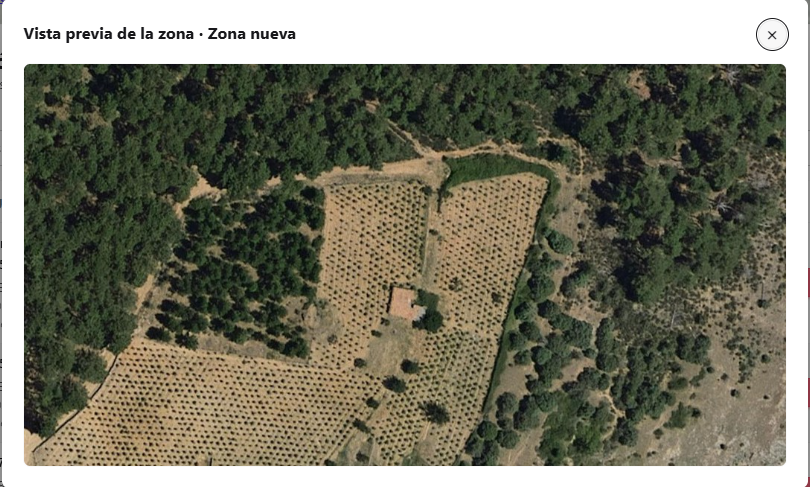
\includegraphics[width=\textwidth]{img/Vista_previa}
	\caption[Vista previa de una colección]{Vista previa de la zona asociada a una colección.}
	\label{fig:manual_vista_previa_coleccion}
\end{figure}

La opción de vista previa permite comprobar visualmente la zona asociada a una colección antes de acceder a sus teselas. Al pulsar el botón correspondiente, se abre una ventana como la mostrada en la Figura~\ref{fig:manual_vista_previa_coleccion}, donde se presenta una imagen general de la zona seleccionada. Esta funcionalidad resulta útil para identificar rápidamente cada colección cuando existen varias zonas registradas.

Desde la columna de acciones, el usuario puede abrir la galería mediante el botón \textit{Ver galería}. Esta vista muestra las teselas individuales generadas para la colección y permite revisar su estado de forma más detallada. También se incluye el botón \textit{Ver en el mapa}, que devuelve al visor cartográfico mostrando la zona seleccionada. Si todas las trazas de la colección ya están calculadas, se habilita un control \textit{Dibujar trazas}, que, al activarlo, representa las trazas directamente sobre la zona descargada.

\begin{figure}[]
	\centering
	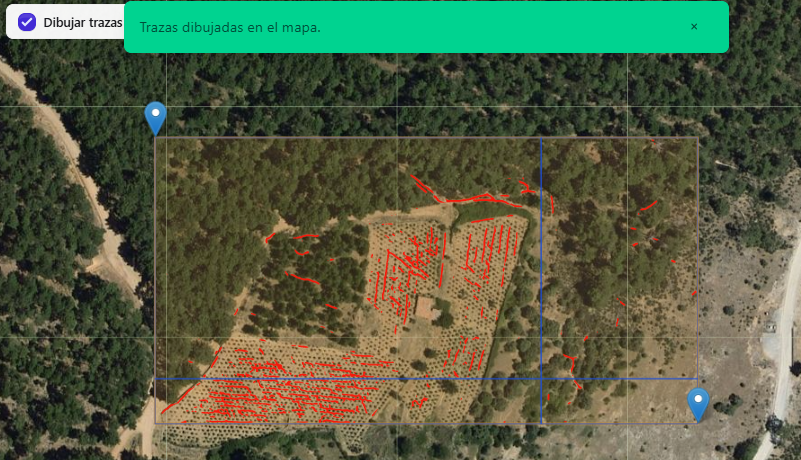
\includegraphics[width=\textwidth]{img/Trazas_mapa}
	\caption[Trazas dibujadas sobre el mapa]{Visualización de las trazas de una colección sobre el visor cartográfico.}
	\label{fig:manual_trazas_mapa}
\end{figure}

La Figura~\ref{fig:manual_trazas_mapa} muestra el resultado de volver al mapa desde una colección y activar la visualización de trazas. En este caso, las detecciones aparecen superpuestas en color rojo sobre la zona seleccionada, manteniendo la referencia espacial de las teselas generadas. Esta opción permite revisar el resultado de la segmentación en su contexto geográfico original.

La colección también permite descargar los resultados en formato \texttt{ZIP}. Esta descarga incluye, para cada tesela procesada correctamente, la imagen original, el resultado generado y el fichero \texttt{JSON} de trazas. Si alguna tesela todavía no tiene las trazas calculadas, se descarga únicamente la imagen original correspondiente. Además, el fichero comprimido incorpora un \texttt{log.json} con información sobre las imágenes descargadas y las posibles descargas fallidas, siguiendo una estructura similar a la siguiente:

\begin{jsonlogbox}{Resultado del proceso de descarga}
	{
		"descargadas": [
		"ma_latest_r01_c01_0.25mpp.jpg",
		"ma_latest_r01_c02_0.25mpp.jpg",
		"ma_latest_r02_c01_0.25mpp.jpg",
		"ma_latest_r02_c02_0.25mpp.jpg"
		],
		"fallidas": []
	}
\end{jsonlogbox}

Por último, esta pantalla permite gestionar las colecciones ya creadas. El usuario puede renombrar una colección para identificarla de forma más clara o eliminarla de forma permanente mediante el botón de borrado. En caso de borrado, la colección deja de aparecer en el listado y se eliminan los recursos asociados según la lógica de la aplicación.

\subsection{Galería de una colección}

La galería de una colección permite revisar de forma individual las teselas generadas para una zona concreta. Desde esta pantalla el usuario puede consultar la información general de la colección, visualizar cada imagen, comprobar el estado de sus trazas, descargar resultados y ejecutar acciones de recalculado cuando sea necesario.

\begin{figure}[]
	\centering
	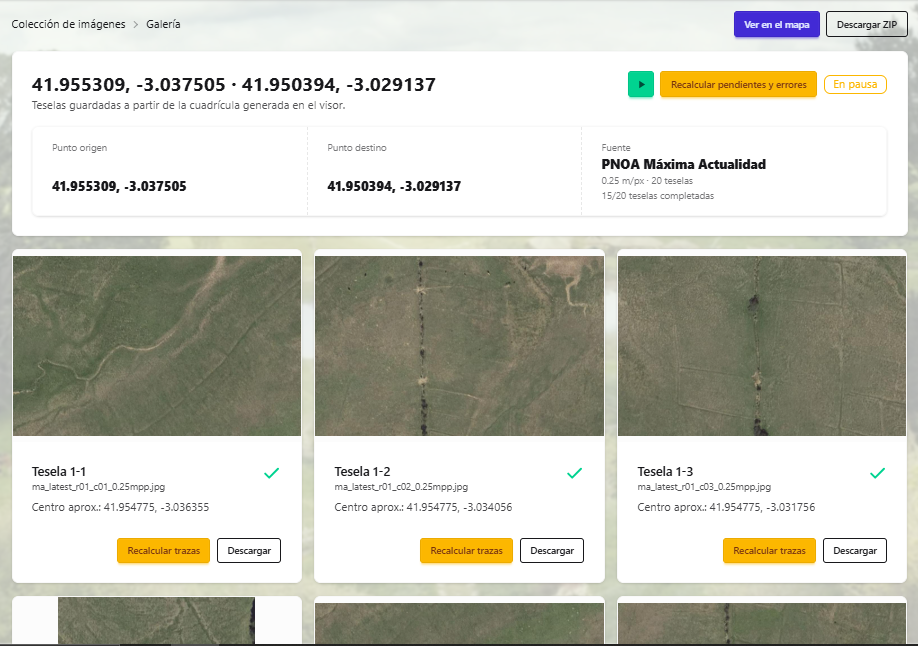
\includegraphics[width=\textwidth]{img/Página_galería}
	\caption[Galería de una colección]{Galería de teselas asociadas a una colección generada desde el visor.}
	\label{fig:manual_galeria}
\end{figure}

Como se observa en la Figura~\ref{fig:manual_galeria}, la parte superior de la pantalla resume los datos principales de la colección, incluyendo las coordenadas de origen y destino, la fuente cartográfica utilizada, la resolución y el número de teselas completadas. También se muestran accesos para volver a la colección, ver la zona en el mapa y descargar el conjunto de resultados. La descarga mantiene la misma lógica descrita en el apartado anterior, por lo que puede incluir imágenes originales, resultados, ficheros \texttt{JSON} y el registro de descarga correspondiente.

Cada tesela aparece representada mediante una tarjeta con su imagen, nombre de archivo, centro aproximado y estado de procesamiento. Los estados posibles coinciden con los de la colección: pendiente, procesando, completada, pausada o error. Esta organización permite revisar rápidamente qué imágenes tienen ya las trazas disponibles y cuáles requieren todavía procesamiento o revisión.

Desde cada tarjeta se puede abrir una vista ampliada de la tesela, descargar únicamente los resultados asociados a esa imagen o recalcular sus trazas. La opción de recalculado individual se habilita pasado un breve margen de tiempo desde el inicio del procesamiento y permite volver a ejecutar el cálculo incluso si la tesela ya estaba completada, lo que resulta útil cuando se desea comprobar de nuevo una imagen concreta.

\begin{figure}[]
	\centering
	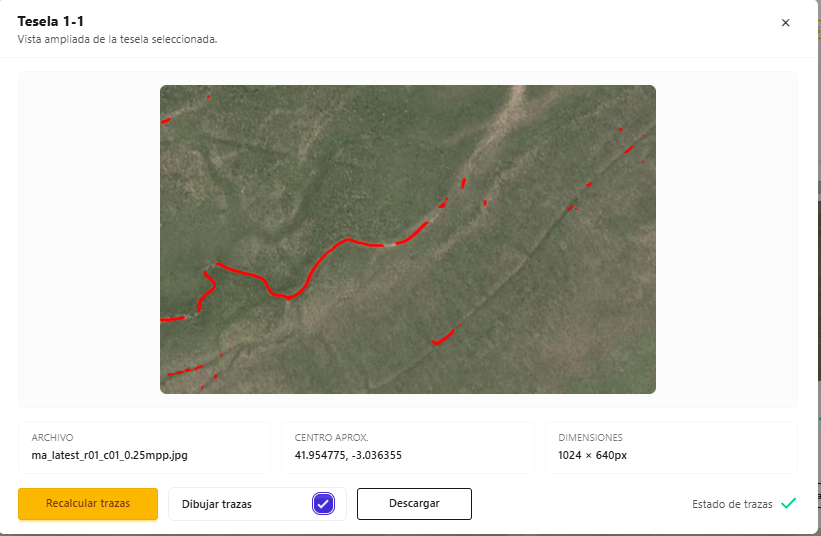
\includegraphics[width=\textwidth]{img/Vista_ampliada}
	\caption[Vista ampliada de una tesela]{Vista ampliada de una tesela con sus trazas calculadas.}
	\label{fig:manual_vista_ampliada}
\end{figure}

La vista ampliada, mostrada en la Figura~\ref{fig:manual_vista_ampliada}, permite inspeccionar una tesela con mayor detalle. En esta pantalla se muestra la imagen seleccionada, sus metadatos principales, el estado de las trazas y varias acciones específicas. El usuario puede activar o desactivar la visualización de trazas mediante el control \textit{Dibujar trazas}; cuando está marcado, las trazas calculadas aparecen superpuestas sobre la imagen, mientras que al desmarcarlo se muestra únicamente la imagen original.

Desde esta vista también es posible descargar solo los ficheros asociados a la tesela seleccionada, sin descargar la colección completa. Además, el botón \textit{Recalcular trazas} permite repetir el procesamiento de esa imagen individual, independientemente del estado del resto de teselas de la colección.

En la galería existe también una acción global de \textit{Recalcular pendientes y errores}. Esta opción está pensada para relanzar únicamente aquellas teselas que hayan quedado pendientes o en estado de error, sin modificar las que ya se han procesado correctamente. El botón aparece inactivo cuando todas las trazas están calculadas correctamente y se habilita tras un breve margen desde el inicio del procesamiento de la colección, evitando acciones prematuras mientras el sistema todavía está trabajando.

Tanto desde la colección como desde la galería, la aplicación permite pausar y reanudar el procesamiento cuando todavía existen teselas pendientes o en curso. Al pulsar el botón de pausa, el cálculo se detiene temporalmente para esa colección y el control cambia visualmente para ofrecer la opción de reanudar. Al reanudar, la aplicación continúa procesando las teselas que quedaban pendientes. Si una colección ya está completada, no se puede pausar, ya que no existe ningún procesamiento activo que detener.

Por último, la galería mantiene acciones de gestión de la colección, como el renombrado, la descarga global y la navegación de vuelta al listado de colecciones o al visor cartográfico. De este modo, el usuario puede moverse entre la visión general de sus zonas, el detalle de una colección y la inspección individual de cada tesela sin perder el contexto del análisis.

\subsection{Cambio de idioma}

La aplicación dispone de soporte multidioma mediante un selector de idioma visible en la interfaz. Este selector permite cambiar los textos principales de la aplicación sin modificar el flujo de uso ni abandonar la pantalla en la que se encuentra el usuario.

\begin{figure}[]
	\centering
	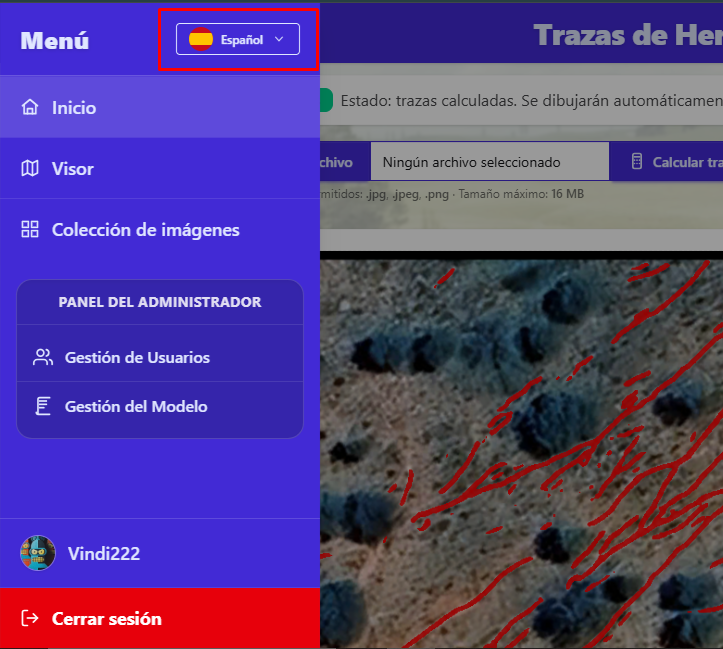
\includegraphics[width=\textwidth]{img/Cambio_idioma}
	\caption[Selector de idioma en la interfaz]{Ubicación del selector de idioma en el menú lateral de la aplicación.}
	\label{fig:manual_cambio_idioma}
\end{figure}

Como se muestra en la Figura~\ref{fig:manual_cambio_idioma}, el selector se encuentra visible en la parte superior de la interfaz, dentro del menú lateral o de la zona de navegación según la pantalla en la que se encuentre el usuario. Al pulsarlo, se despliega una lista con los idiomas disponibles.

\begin{figure}[]
	\centering
	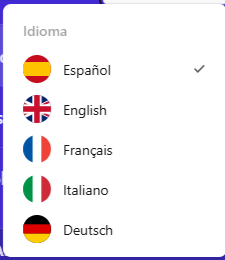
\includegraphics[width=0.35\textwidth]{img/Selector_idioma}
	\caption[Idiomas disponibles]{Lista de idiomas disponibles en el selector de la aplicación.}
	\label{fig:manual_selector_idioma}
\end{figure}

En la Figura~\ref{fig:manual_selector_idioma} se observa el desplegable de idiomas. Desde esta lista el usuario puede seleccionar el idioma deseado, por ejemplo español, inglés, francés, italiano o alemán. El idioma actualmente activo aparece marcado, lo que permite identificar rápidamente la configuración aplicada en ese momento.

\begin{figure}[]
	\centering
	\includegraphics[width=\textwidth]{img/imagen_inglés}
	\caption[Interfaz en inglés]{Página principal de la aplicación tras seleccionar el idioma inglés.}
	\label{fig:manual_idioma_ingles}
\end{figure}

Cuando se cambia el idioma, los textos visibles de la aplicación pasan a mostrarse en la lengua seleccionada, como se aprecia en la Figura~\ref{fig:manual_idioma_ingles}. Esto afecta a botones, mensajes de estado, avisos, formularios y demás elementos textuales de la interfaz. La preferencia de idioma se mantiene durante la sesión, de forma que el usuario puede seguir navegando por la aplicación con la misma configuración lingüística mientras continúe utilizando el sistema.

\subsection{Mensajes de error y validación}

La aplicación informa al usuario mediante mensajes de validación, avisos y modales cuando una operación no puede completarse, cuando requiere confirmación o cuando finaliza correctamente. Estos mensajes aparecen de forma visible en la interfaz y permiten comprender rápidamente qué ha ocurrido y qué acción debe realizarse a continuación.

\begin{figure}[]
	\centering
	
\includegraphics[width=0.75\textwidth]{img/Warning_selección}
	\caption[Aviso de selección activa]{Aviso mostrado cuando ya existe una selección activa en el visor.}
	\label{fig:manual_warning_seleccion}
\end{figure}

Los avisos se utilizan para situaciones en las que la acción no es necesariamente un error, pero el usuario debe modificar el flujo antes de continuar. Por ejemplo, si ya existe una selección activa en el visor, la aplicación muestra un mensaje como el de la Figura~\ref{fig:manual_warning_seleccion}, indicando que debe utilizarse la opción \textit{Reiniciar selección} antes de comenzar una nueva.

\begin{figure}[]
	\centering
	\includegraphics[width=0.75\textwidth]{img/error_img_individual}
	\caption[Error al calcular trazas sin imagen]{Mensaje de error mostrado al intentar calcular trazas sin haber cargado una imagen.}
	\label{fig:manual_error_img_individual}
\end{figure}

Los errores aparecen cuando una operación no puede ejecutarse correctamente. En el flujo de imagen individual, por ejemplo, si el usuario pulsa \textit{Calcular trazas} sin haber seleccionado antes una imagen, la aplicación muestra un mensaje de error como el de la Figura~\ref{fig:manual_error_img_individual}. También pueden aparecer errores si el fichero seleccionado no tiene un formato válido, si supera el tamaño permitido o si se produce algún problema durante el procesamiento.

\begin{figure}[]
	\centering
	\includegraphics[width=0.8\textwidth]{img/error_visor}
	\caption[Error en el visor cartográfico]{Mensaje de error mostrado cuando no existe cobertura cartográfica adecuada para la zona seleccionada.}
	\label{fig:manual_error_visor}
\end{figure}

En el visor cartográfico, los mensajes de error se emplean para informar de problemas relacionados con la zona seleccionada o con los servicios cartográficos. Por ejemplo, si no se encuentra cobertura PNOA adecuada para el área elegida, se muestra un aviso como el de la Figura~\ref{fig:manual_error_visor}. De forma similar, la aplicación puede advertir si la zona seleccionada no es válida, si se encuentra fuera de los límites admitidos o si no es posible generar correctamente la colección.

Además de los errores de imagen y visor, la aplicación también valida otros flujos de uso. Si las credenciales introducidas en el inicio de sesión son incorrectas, se informa al usuario para que revise el nombre de usuario y la contraseña. En la gestión de modelos, si un modelo subido no supera la validación, no queda disponible para su uso y se muestra el mensaje correspondiente al administrador. Asimismo, si una colección no contiene datos disponibles o no tiene resultados calculados, la interfaz lo comunica para evitar que el usuario intente visualizar o descargar información inexistente.

\begin{figure}[]
	\centering
	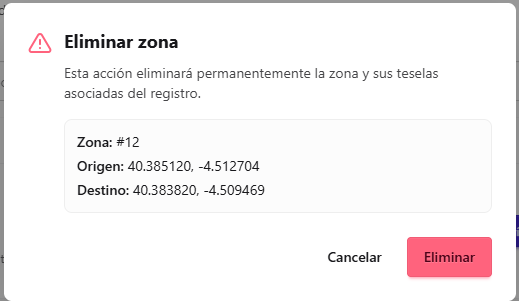
\includegraphics[width=0.8\textwidth]{img/Confirmación_borrado}
	\caption[Confirmación de borrado de una colección]{Modal de confirmación para validar la eliminación de una entrada de la colección.}
	\label{fig:conf_borrado}
\end{figure}

Algunas acciones requieren confirmación previa, especialmente aquellas que eliminan información, como se puede ver en la Figura~\ref{fig:conf_borrado}. Por ejemplo, al borrar una imagen, una colección o un usuario desde administración, la aplicación puede mostrar un modal de confirmación antes de ejecutar la operación definitiva. Este comportamiento evita borrados accidentales y permite al usuario cancelar la acción si no está seguro.

\begin{figure}[]
	\centering
	\includegraphics[width=0.45\textwidth]{img/modal_borrado_img_satisfactorio_inglés}
	\caption[Mensaje de operación completada]{Mensaje de confirmación mostrado tras completar correctamente una acción.}
	\label{fig:manual_accion_correcta}
\end{figure}

Por último, la aplicación también muestra mensajes de confirmación cuando una operación se completa correctamente. Estos mensajes, como el de la Figura~\ref{fig:manual_accion_correcta}, que en este caso ha sido traducido con el selector de idioma, aparecen tras acciones como borrar una imagen, guardar cambios, registrar una zona, calcular trazas o actualizar información del perfil. De este modo, el usuario recibe una retroalimentación clara sobre el resultado de cada operación.

\section{Manual del administrador}

En este apartado se describen las funcionalidades reservadas a los usuarios con rol administrador, orientadas a la gestión interna de usuarios y modelos de la aplicación.

\subsection{Administración de usuarios}

Los usuarios con rol administrador pueden acceder a un panel de gestión desde el que consultar, editar y eliminar las cuentas registradas en la aplicación. Esta sección solo aparece disponible para administradores, tanto desde el menú lateral como desde el perfil de usuario, evitando que los usuarios normales puedan acceder a operaciones de mantenimiento del sistema.

\begin{figure}[]
	\centering
	\includegraphics[width=\textwidth]{img/página_gest_usu}
	\caption[Panel de gestión de usuarios]{Panel de administración para la gestión de usuarios registrados.}
	\label{fig:manual_gestion_usuarios}
\end{figure}

Como se muestra en la Figura~\ref{fig:manual_gestion_usuarios}, la pantalla de gestión presenta un resumen general con el número total de usuarios, administradores y usuarios regulares. Debajo se incluye el listado completo de cuentas registradas, donde se muestran datos como el identificador, nombre de usuario, correo electrónico, teléfono, rol, fecha de registro e imagen o avatar asociado a cada cuenta.

La tabla incorpora un buscador que permite filtrar usuarios por distintos campos, como nombre, correo electrónico, teléfono o rol. También dispone de un selector para modificar el número de registros visibles, facilitando la consulta cuando existen muchas cuentas en el sistema. Además, el administrador puede exportar el estado actual del listado en formato \texttt{CSV} o \texttt{PDF}, lo que permite conservar una copia externa de la información mostrada.

Desde la columna de acciones, el administrador puede ver el detalle de un usuario, editar su información o iniciar el proceso de eliminación. La opción \textit{Ver} permite acceder a una pantalla específica con la información completa de la cuenta seleccionada.

\begin{figure}[]
	\centering
	\includegraphics[width=\textwidth]{img/ver_usu}
	\caption[Detalle de usuario]{Vista de detalle de un usuario registrado desde el panel de administración.}
	\label{fig:manual_ver_usuario}
\end{figure}

En la Figura~\ref{fig:manual_ver_usuario} se muestra la vista de detalle de un usuario. Desde esta pantalla el administrador puede consultar la imagen de perfil, el identificador, correo electrónico, teléfono, fecha de alta, rol y número de parcelas asociadas. También se incluyen accesos para volver al listado, editar el usuario o eliminar la cuenta.

\begin{figure}[]
	\centering
	\includegraphics[width=\textwidth]{img/editar_usu}
	\caption[Edición de usuario]{Formulario de edición de usuario desde el panel de administración.}
	\label{fig:manual_editar_usuario}
\end{figure}

La opción \textit{Editar} abre el formulario representado en la Figura~\ref{fig:manual_editar_usuario}. Desde esta vista el administrador puede modificar datos visibles del usuario, como el nombre, el correo electrónico, el teléfono y, cuando procede, el rol. En el caso de cuentas administradoras protegidas, la aplicación informa de que el rol no puede modificarse desde esta vista, evitando cambios accidentales sobre permisos críticos.

La eliminación de usuarios se realiza mediante una acción específica de borrado y requiere confirmación antes de ejecutarse. Este paso evita eliminaciones accidentales, ya que la operación afecta a una cuenta registrada y puede implicar la pérdida de acceso del usuario al sistema. Una vez confirmada la eliminación, el usuario deja de aparecer en el listado de administración.

\subsection{Administración de modelos}

La gestión de modelos permite controlar qué modelos de segmentación están disponibles en la aplicación y cuál de ellos se utilizará para realizar las inferencias. Esta funcionalidad está reservada exclusivamente a usuarios con rol administrador, ya que afecta directamente al comportamiento del sistema durante el cálculo de trazas.

\begin{figure}[]
	\centering
	\includegraphics[width=\textwidth]{img/página_gest_modelo}
	\caption[Panel de gestión de modelos]{Panel de administración para la gestión de modelos de segmentación.}
	\label{fig:manual_gestion_modelos}
\end{figure}

Como se observa en la Figura~\ref{fig:manual_gestion_modelos}, esta pantalla muestra un listado con los modelos registrados en el sistema. Para cada uno de ellos se indica su identificador, nombre, estado, validación y fecha de creación. El estado permite saber si el modelo está activo o no, mientras que la validación indica si el modelo ha superado correctamente la comprobación previa necesaria para poder utilizarse.

El modelo marcado como activo es el que utiliza la aplicación para realizar nuevas inferencias, tanto sobre imágenes individuales como sobre teselas generadas desde el visor cartográfico. Por este motivo, solo debe activarse un modelo que haya sido validado correctamente. Desde la columna de acciones, el administrador puede activar un modelo, renombrarlo o eliminarlo, siempre que la operación esté permitida por el estado actual del modelo.

\begin{figure}[]
	\centering
	\includegraphics[width=0.65\textwidth]{img/añadir_modelo}
	\caption[Formulario para añadir modelo]{Formulario de subida de un nuevo modelo de segmentación.}
	\label{fig:manual_anadir_modelo}
\end{figure}

Para incorporar un nuevo modelo, el administrador debe pulsar el botón \textit{Añadir modelo}. A continuación, se abre el formulario mostrado en la Figura~\ref{fig:manual_anadir_modelo}, donde se solicita un nombre identificativo y el archivo correspondiente al modelo. El nombre debe ser único y no debe contener rutas ni caracteres reservados del sistema.

Tras guardar el archivo, el modelo queda inicialmente en estado pendiente y se inicia su validación en segundo plano. Durante este proceso, la aplicación comprueba que el modelo puede cargarse y ejecutar una inferencia de prueba. Si la validación finaliza correctamente, el modelo pasa a figurar como validado y podrá ser activado por el administrador. Si la validación falla, el sistema informa del problema y el modelo no queda disponible para inferencia.

La opción de renombrado permite modificar el nombre visible de un modelo sin alterar su función dentro del sistema. Por su parte, la fecha de creación permite identificar cuándo fue incorporado cada modelo, facilitando el seguimiento de versiones y la gestión de distintos artefactos de segmentación. De este modo, el panel de administración ofrece un control centralizado sobre los modelos disponibles y sobre el modelo activo utilizado por la aplicación.

